\documentclass[xcolor=dvipsnames]{beamer}

\usepackage{graphicx}
\usepackage{wrapfig}
\usepackage{colortbl}
\definecolor{myblue}{rgb}{0.8,0.85,1}

\mode<presentation>
{
  \usetheme{Warsaw}
  \setbeamercovered{transparent}
}
% \usecolortheme[named=OliveGreen]{structure}
\setbeamertemplate{navigation symbols}{} 
\setbeamertemplate{blocks}[rounded][shadow=true] 

\title{The Full Employment Theory \linebreak in Probability Kinematics}
\subtitle{Gesellschaft f{\"u}r Wissenschaftsphilosophie}

\author{Stefan Lukits, University of British Columbia}

\date{March 13, 2013}

% \logo{
\includegraphics[height=.8cm]{photo1.jpg}}

\begin{document}

\begin{frame}
  \titlepage
\end{frame}

\begin{frame}
  \frametitle{Probability Kinematics}
  You have a fully quantified probability assessment of an event
  space. You make an observation. What is the most rationally
  defensible way of updating your probabilities? Three cases:
  \begin{enumerate}
  \item The observation is an event.
  \item The observation redistributes the probabilities of a
    partition of the event space.
  \item The observation is an affine constraint.
  \end{enumerate}
\end{frame}

\begin{frame}
  \frametitle{Conditioning}
  Example: Hercule Poirot considers the probabilities as he
  investigates the murder of Roger Ackroyd. He observes that the
  culprit must have been male.

\mbox{}

\mbox{}

  \begin{tabular}{|l|r|r|} \hline
    Mrs. Cecil Ackroyd, the sister-in-law & 0.08 & 0.00 \\ \hline
    Flora Ackroyd, her daughter & 0.08 & 0.00 \\ \hline
    Major Blunt, a big-game hunter & 0.08 & 0.11 \\ \hline
    Geoffrey Raymond, the personal secretary & 0.08 & 0.11 \\ \hline
    Ralph Paton, the stepson with heavy debts & 0.52 & 0.68 \\ \hline
    Parker, the snooping butler & 0.08 & 0.11 \\ \hline
    Ursula Bourne, the parlour maid & 0.08 & 0.00 \\ \hline
  \end{tabular}
\end{frame}

\begin{frame}
  \frametitle{Jeffrey Conditioning}
  Example: Hercule Poirot considers the probabilities as he
  investigates the murder of Roger Ackroyd. He observes that the
  chance of the culprit being male is only 1/2.

\mbox{}

\mbox{}

  \begin{tabular}{|l|r|r|} \hline
    Mrs. Cecil Ackroyd, the sister-in-law & 0.08 & 0.17 \\ \hline
    Flora Ackroyd, her daughter & 0.08 & 0.17 \\ \hline
    Major Blunt, a big-game hunter & 0.08 & 0.05 \\ \hline
    Geoffrey Raymond, the personal secretary & 0.08 & 0.05 \\ \hline
    Ralph Paton, the stepson with heavy debts & 0.52 & 0.34 \\ \hline
    Parker, the snooping butler & 0.08 & 0.05 \\ \hline
    Ursula Bourne, the parlour maid & 0.08 & 0.17 \\ \hline
  \end{tabular}
\end{frame}

\begin{frame}
  \frametitle{Affine Constraint}
  Example: Hercule Poirot considers the probabilities as he
  investigates the murder of Roger Ackroyd. He observes that the
  chance of Ralph Paton being the culprit is twice as high as the
  chance of Major Blunt being the culprit.

\mbox{}

  \begin{tabular}{|l|r|r|} \hline
    Mrs. Cecil Ackroyd, the sister-in-law & 0.08 & ?.?? \\ \hline
    Flora Ackroyd, her daughter & 0.08 & ?.?? \\ \hline
    Major Blunt, a big-game hunter & 0.08 & ?.?? \\ \hline
    Geoffrey Raymond, the personal secretary & 0.08 & ?.?? \\ \hline
    Ralph Paton, the stepson with heavy debts & 0.52 & ?.?? \\ \hline
    Parker, the snooping butler & 0.08 & ?.?? \\ \hline
    Ursula Bourne, the parlour maid & 0.08 & ?.?? \\ \hline
  \end{tabular}
\end{frame}

\begin{frame}
  \frametitle{The Principle of Maximum Entropy}
\begin{figure}[h]
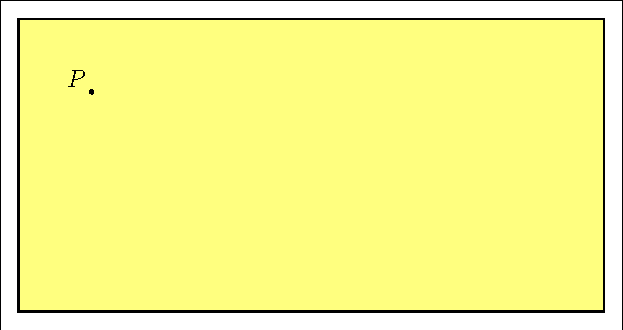
\includegraphics[scale=1.0]{../diagrams/constraint-a.pdf}
\end{figure}
\end{frame}

\begin{frame}
  \frametitle{The Principle of Maximum Entropy}
\begin{figure}[h]
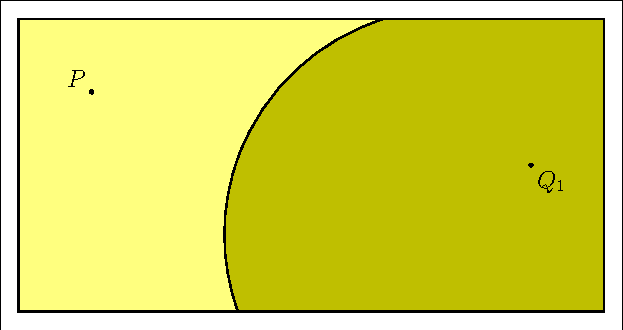
\includegraphics[scale=1.0]{../diagrams/constraint-b.pdf}
\end{figure}
\end{frame}

\begin{frame}
  \frametitle{The Principle of Maximum Entropy}
\begin{figure}[h]
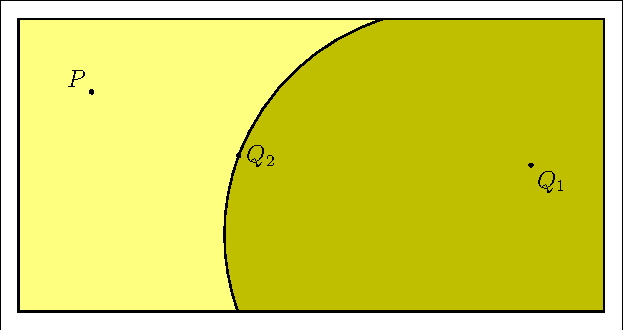
\includegraphics[scale=1.0]{../diagrams/constraint-c.pdf}
\end{figure}
\end{frame}

\begin{frame}
  \frametitle{The Principle of Maximum Entropy}
\begin{figure}[h]
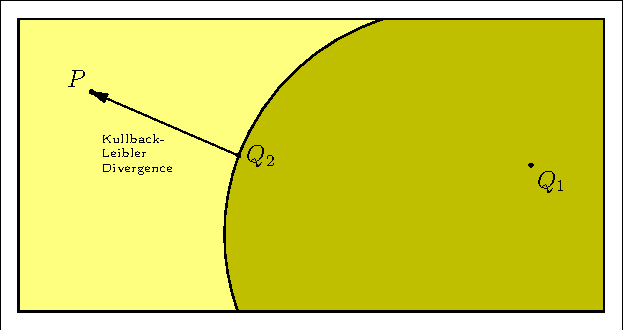
\includegraphics[scale=1.0]{../diagrams/constraint-d.pdf}
\end{figure}
\end{frame}

\begin{frame}
  \frametitle{Principle of Maximum Entropy vs. Full Employment I}
\begin{itemize}
\item Shore and Johnson (1980) show that, under certain
  assumptions, there is a unique solution to the problem of
  updating probabilities under an affine constraint. The Principle
  of Maximum Entropy: given an affine constraint, the updated
  probability assignment is the one that is both consistent with
  the constraint and informationally minimally distant from the
  prior probability assignment.
\end{itemize}
\end{frame}

\begin{frame}
  \frametitle{Principle of Maximum Entropy vs. Full Employment II}
\begin{itemize}
\item Enter the Full Employment Theorem. Shore and Johnson's
  assumptions are not unanimously endorsed (see especially Uffink
  1995). There are examples where the Principle of Maximum Entropy
  results in counterintuitive probability updating, most
  prominently the Judy Benjamin case.
\item Consequently, there is an array of solutions and no
  objective method to decide between them. Only a subjective
  assessment of the situation can narrow down the solution space.
\item We will undermine the notion that the results of the
  examples are counterintuitive, specifically with respect to
  independence, the powerset approach, epistemic entrenchment, and
  coarsening at random.
\end{itemize}
\end{frame}

\begin{frame}
  \frametitle{Principle of Maximum Entropy vs. Full Employment III}
  \begin{block}{Principle of Maximum Entropy}
    ``Jaynes's principle of maximum entropy and Kullbacks
    principle of minimum cross-entropy (minimum directed
    divergence) are shown to be uniquely correct methods for
    inductive inference when new information is given in the form
    of expected values.'' \linebreak (Shore and Johnson)
  \end{block}
  \begin{block}{Full Employment}
    ``The uniqueness proofs are flawed, or rest on unreasonably
    strong assumptions. A more general class of inference rules,
    maximizing the so-called R{\'e}nyi entropies, is exhibited
    which also fulfill the reasonable part of the consistency
    assumptions.'' (Jos Uffink)
  \end{block}
\end{frame}

\begin{frame}
  \frametitle{Principle of Maximum Entropy vs. Full Employment IV}
  \begin{block}{Principle of Maximum Entropy}
    ``We show that Skilling's method of induction leads us to a
    unique general theory of inductive inference, the maximum
    entropy method, and precisely how it is that other entropies
    such as those of R{\'e}nyi or Tsallis are ruled out for
    problems of inference. We then explore the compatibility of
    Bayes and maximum entropy updating. We show that maximum
    entropy is capable of producing every aspect of orthodox
    Bayesian inference and prove the complete compatibility of
    Bayesian and entropy methods.'' (Adom Giffin)
 \end{block}
\end{frame}

\begin{frame}
  \frametitle{Principle of Maximum Entropy vs. Full Employment V}
\begin{block}{Full Employment}
  ``Maximum entropy and relative entropy have proved quite
  successful in a number of applications, from physics to
  natural-language modeling. Unfortunately, they also exhibit some
  counterintuitive behavior on certain applications. Although they
  are valuable tools, they should be used with care.'' \linebreak
  (Joseph Halpern)
\end{block}
\end{frame}

\begin{frame}
  \frametitle{Halpern's Full Employment Theorem}
  \begin{columns}
    \column{.50\textwidth}{
Choosing a representation:
    \begin{itemize}
    \item possible worlds
    \item probability measures
    \item lower and upper probabilities
    \item Dempster-Shafer belief functions
    \item possibility measures
    \item ranking functions
    \item relative likelihoods
    \item plausibility measures
    \end{itemize}}
\column{.50\textwidth}{
  \begin{block}{Grove and Halpern}
    ``one must always think carefully about precisely what the
    information means'' \linebreak (``Probability Update \ldots,'' p6)
  \end{block}
  \begin{block}{Joseph Halpern}
    ``there is no escaping the need to understand the details of the
    application'' \linebreak (\emph{Reasoning \ldots}, p423)
  \end{block}
}
  \end{columns}
\end{frame}

\begin{frame}
  \frametitle{The Judy Benjamin Case I}
\begin{figure}[h]
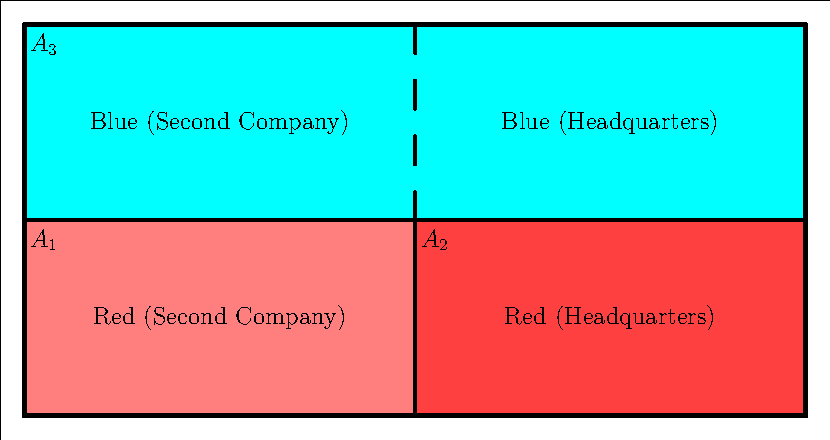
\includegraphics[scale=.7]{../diagrams/judy.pdf}
\end{figure}
\end{frame}

\begin{frame}
  \frametitle{The Judy Benjamin Case II}
\begin{itemize}
\item (MAP) Judy has no idea where she is. She is on team Blue.
  Because of the map, her probability of being in Blue territory
  equals the probability of being in Red territory, and being on Red
  Second Company ground equals the probability of being on Red
  Headquarters ground.
\item (HDQ) Headquarters inform Judy that in case she is in Red
  territory, her chance of being on their Headquarters ground is three
  times the chance of being on their Second Company ground.
\end{itemize}
\begin{equation}
  \label{eq:map}
  2\cdot{}P(A_{1})=2\cdot{}P(A_{2})=P(A_{3})\tag{\mbox{MAP}}
\end{equation}
\begin{equation}
  \label{eq:hdq}
  q=P(A_{2}|A_{1}\cup{}A_{2})=\frac{3}{4}\tag{\mbox{HDQ}}
\end{equation}
\end{frame}

\begin{frame}
  \frametitle{Two Intuitions}
  \begin{itemize}
  \item<1->[\color{blue}{(T1)}] HDQ should not affect $P(A_{3})$. Let's
    call $P$ the prior probability distribution, before receiving HDQ,
    and $Q$ the posterior probability distribution, after receiving
    HDQ. Then $Q(A_{3})=P(A_{3})$.
  \item<2->[\color{blue}{(T2)}] If the value of $q$ approaches $1$
  then $Q(A_{3})$ should approach $2/3$. HDQ would then be ``if you
  are in Red territory you are almost certainly on Red Headquarters
  ground.'' Considering MAP, $Q(A_{3})$ should approach $2/3$.
  Continuity considerations pose a contradiction to T1.
  \end{itemize}
\end{frame}

\begin{frame}
  \frametitle{The PME Applied to Judy Benjamin}
Intuition T1: use the space originally occupied by the affected
probabilities and redistribute it:
  \begin{displaymath}
    v_{1}=(0.125,0.375,0.500)
  \end{displaymath}

Intuition T2: use the constraint rule to determine which
probability assignment is consistent with the the constraint
while minimizing the informational divergence with the prior
probability:
  \begin{displaymath}
    v_{2}\approx{}(0.117,0.350,0.533)
  \end{displaymath}
\end{frame}

\begin{frame}
  \frametitle{Intuition T1}
\begin{figure}[h]
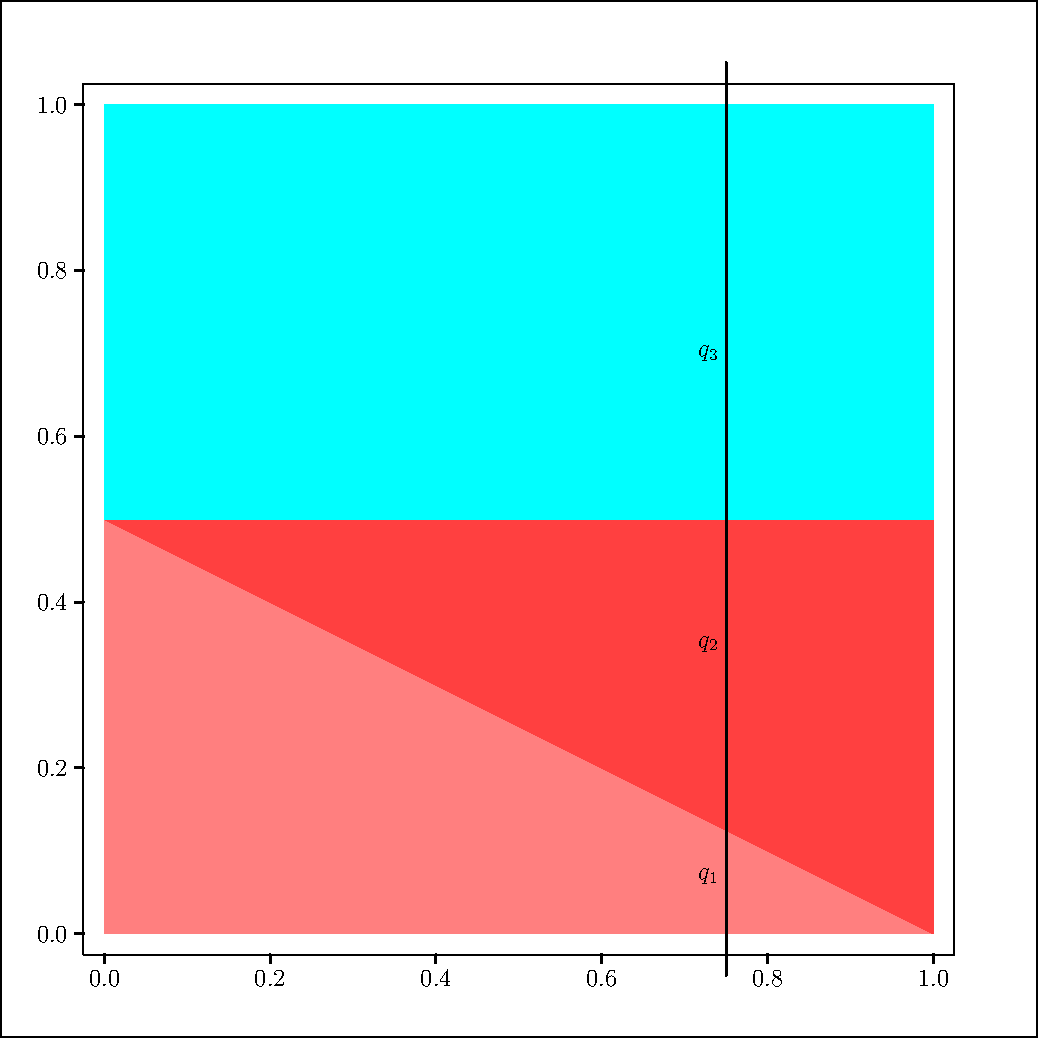
\includegraphics[scale=.4]{../diagrams/zeroone-unif.pdf}
\end{figure}
\end{frame}

\begin{frame}
  \frametitle{Intuition T2}
\begin{figure}[h]
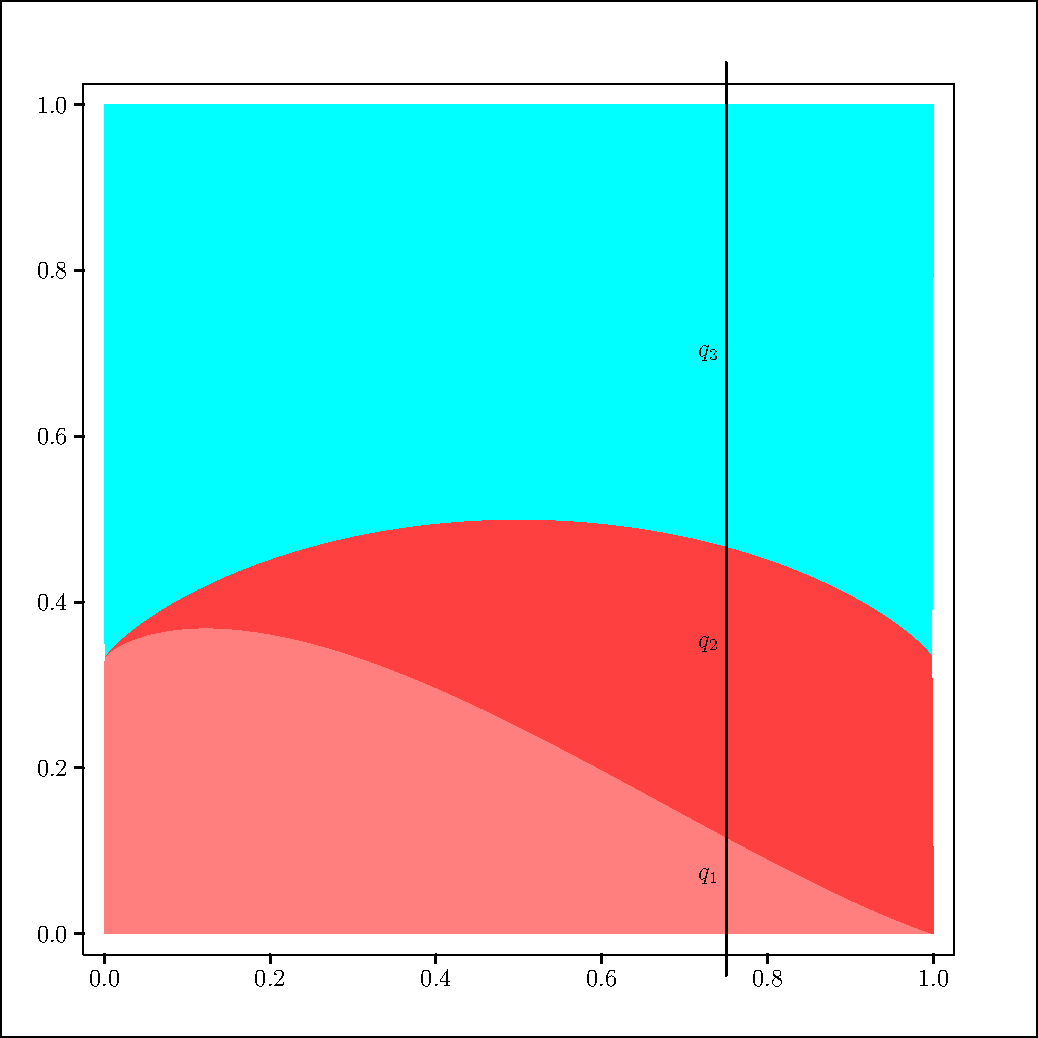
\includegraphics[scale=.4]{../diagrams/zeroone-mxnt.pdf}
\end{figure}
\end{frame}

\begin{frame}
  \frametitle{Four Scenarios I}
  Here are four scenarios, in which Judy may have received
  ({\ref{eq:hdq}}):
\begin{enumerate}
\item[S1] Judy was dropped off by a pilot who flipped two coins. If
  the first coin landed H, then Judy was dropped off in Blue
  territory, otherwise in Red territory. If the second coin landed H,
  she was dropped off on Headquarters ground, otherwise on Second
  Company ground. Judy's headquarters find out that the second coin
  was biased $q:1-q$ toward H. The normalized odds vector is
  $v=(.125,.375,.5)$ and agrees with (T1), because the choice of Blue
  or Red is completely independent from the choice of Headquarters or
  Second Company.
\end{enumerate}
\end{frame}

\begin{frame}
  \frametitle{Four Scenarios II}
\begin{enumerate}
\item [S2] Judy's Headquarters has divided the map into $24$ congruent
  rectangles, $A_{3}$ into twelve, and $A_{1}$ and $A_{2}$ into six
  rectangles each. They have information that the only subsets of the
  $24$ rectangles in which Judy Benjamin may be located are such that
  they contain three times as many $A_{2}$ rectangles than $A_{1}$
  rectangles. Thus they relay ({\ref{eq:hdq}}) to Judy, which she
  correctly interprets with the normalized odds vector
  $v=(.108,.324,.568)$ (evaluating the $16777216$ subsets).
\end{enumerate}
\end{frame}

\begin{frame}
  \frametitle{Four Scenarios III-IV}
\begin{enumerate}
\item[S3] The pilot randomly lands in any of the four quadrants and
  rolls a die. If she rolls an even number, she drops off Judy. If
  not, she takes her to another (or the same) randomly selected
  quadrant to repeat the procedure. Headquarters find out, however,
  that for $A_{1}$, the pilot requires a six to drop off Judy, not
  just an even number. Thus they relay ({\ref{eq:hdq}}) to Judy, which
  she correctly interprets with the normalized odds vector
  $v=(.1,.3,.6)$.
\item [S4] Judy's headquarters know that Judy is not in $A_{3}$ and
  that her chance of being in $A_{2}$ is three times the chance of
  being in $A_{1}$. They only succeed, however, in informing Judy of
  the second part of the message. If Judy had all the information, her
  normalized odds vector would be $v=(.33,.67,0)$.
\end{enumerate}
\end{frame}

\begin{frame}
  \frametitle{Powerset Approach I}
  Reconsider Scenario S2: Judy's Headquarters has divided the map
  into $24$ congruent rectangles, $A_{3}$ into twelve, and $A_{1}$
  and $A_{2}$ into six rectangles each. They have information that
  the only subsets of the $24$ rectangles in which Judy Benjamin
  may be located are such that they contain three times as many
  $A_{2}$ rectangles than $A_{1}$ rectangles. Thus they relay
  ({\ref{eq:hdq}}) to Judy, which she correctly interprets with
  the normalized odds vector $v=(.108,.324,.568)$ (evaluating the
  $16777216$ subsets).

\mbox{}

  Now let the grain of this partition become infinitely small.
  There are strong independence and uniformity assumptions at work
  here. It is reasonable to predict that the results of the
  powerset approach will support intuition T1.
\end{frame}

\begin{frame}
  \frametitle{Powerset Approach II}
\begin{figure}[h]
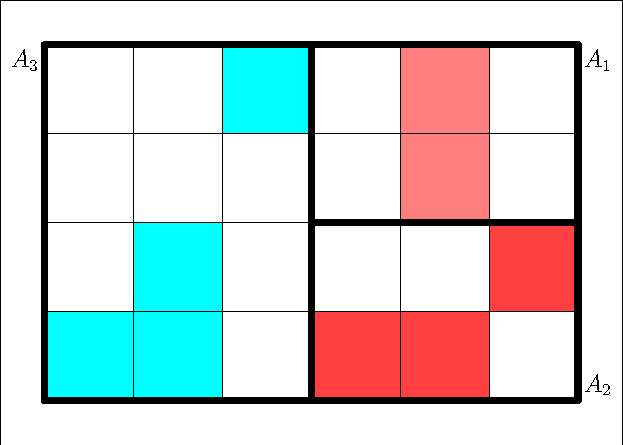
\includegraphics[scale=.7]{../diagrams/partition-2.pdf}
\end{figure}
\end{frame}

\begin{frame}
  \frametitle{Powerset Approach III}
\begin{figure}[h]
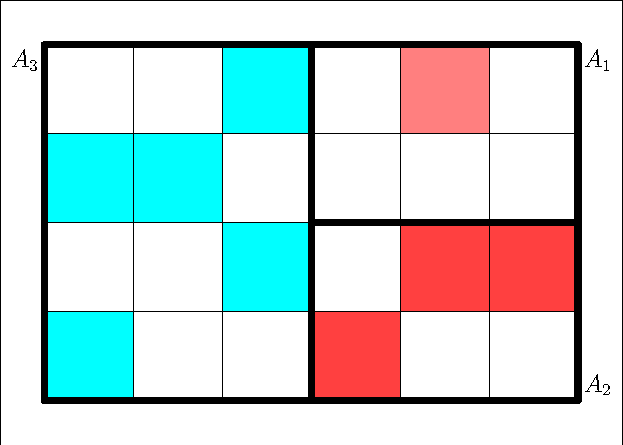
\includegraphics[scale=.7]{../diagrams/partition-1.pdf}
\end{figure}
\end{frame}

\begin{frame}
  \frametitle{Intuition T1}
\begin{figure}[h]
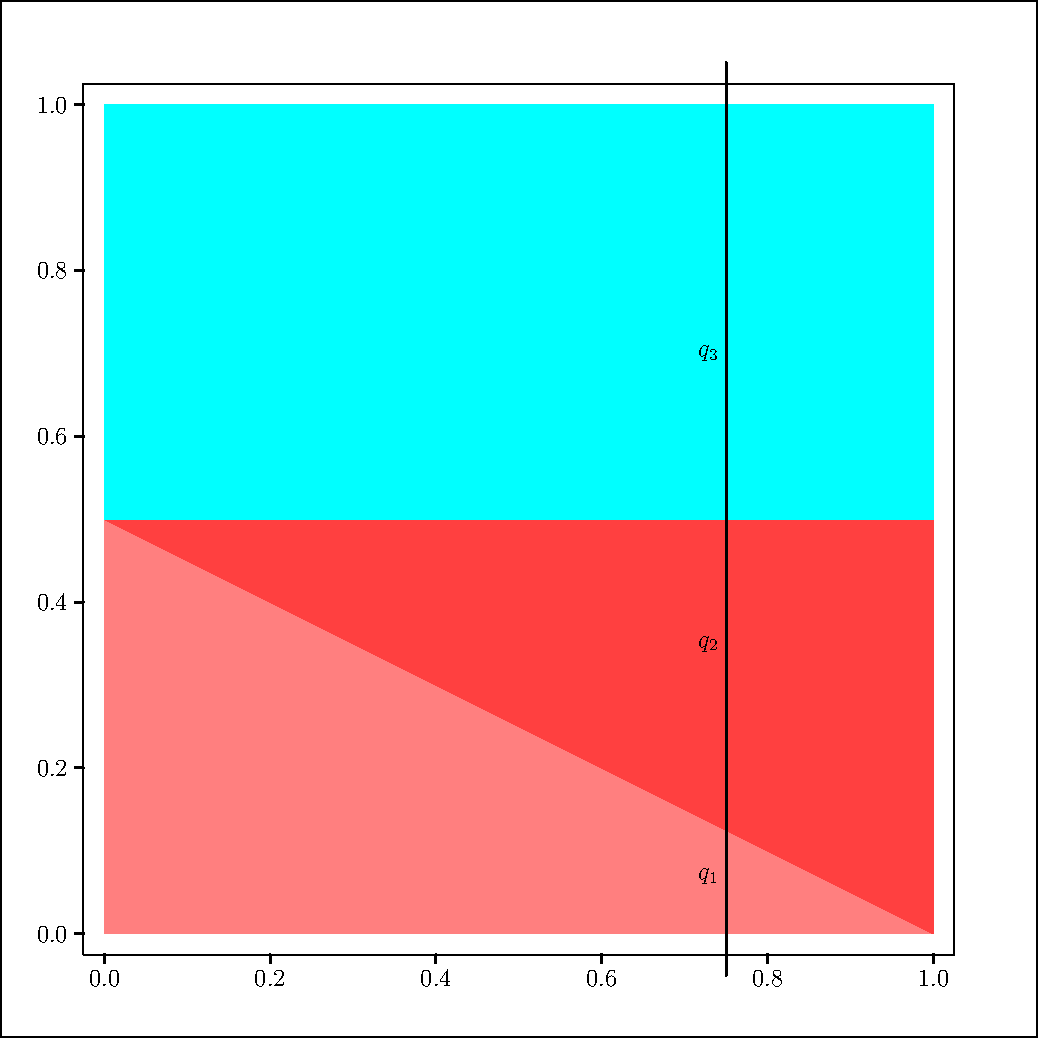
\includegraphics[scale=.4]{../diagrams/zeroone-unif.pdf}
\end{figure}
\end{frame}

\begin{frame}
  \frametitle{Intuition T2}
\begin{figure}[h]
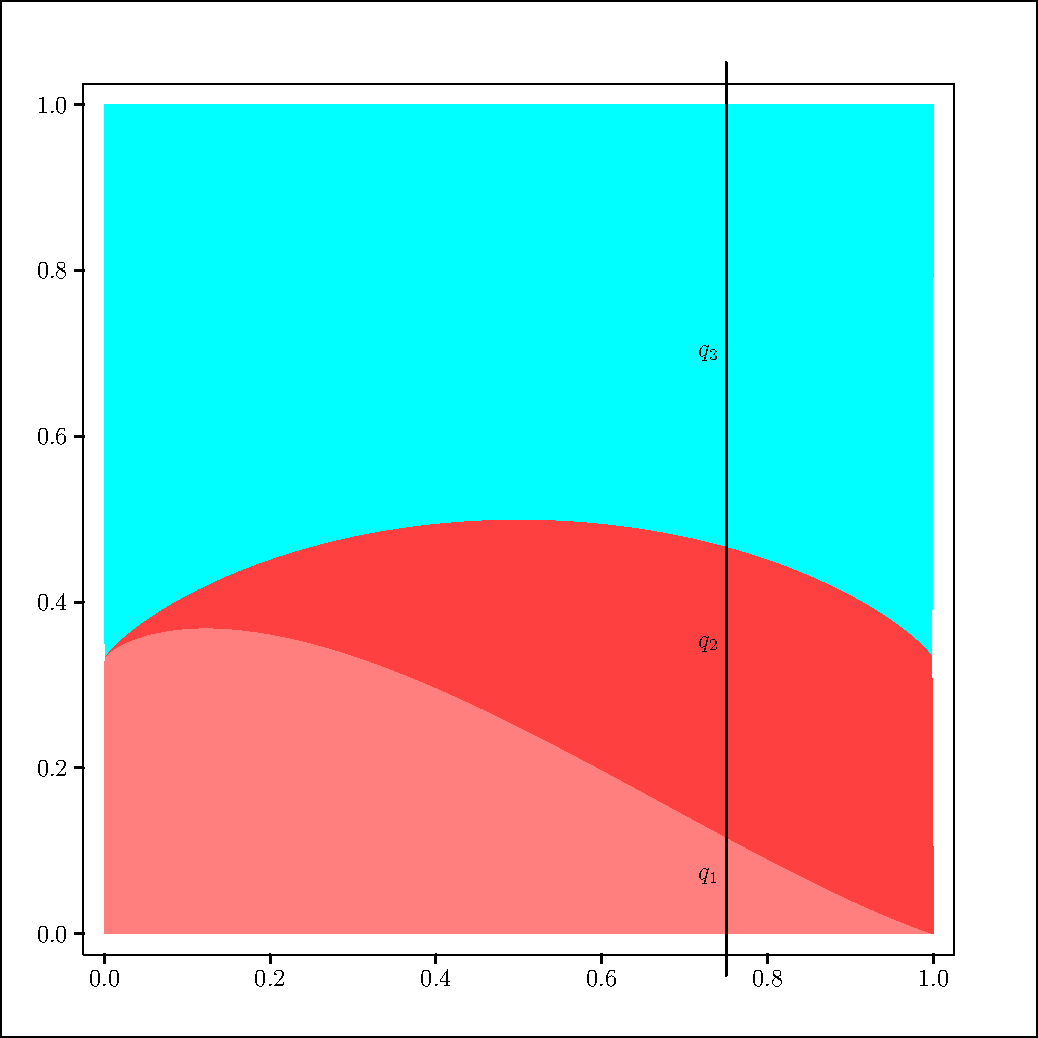
\includegraphics[scale=.4]{../diagrams/zeroone-mxnt.pdf}
\end{figure}
\end{frame}

\begin{frame}
  \frametitle{Powerset Approach}
\begin{figure}[h]
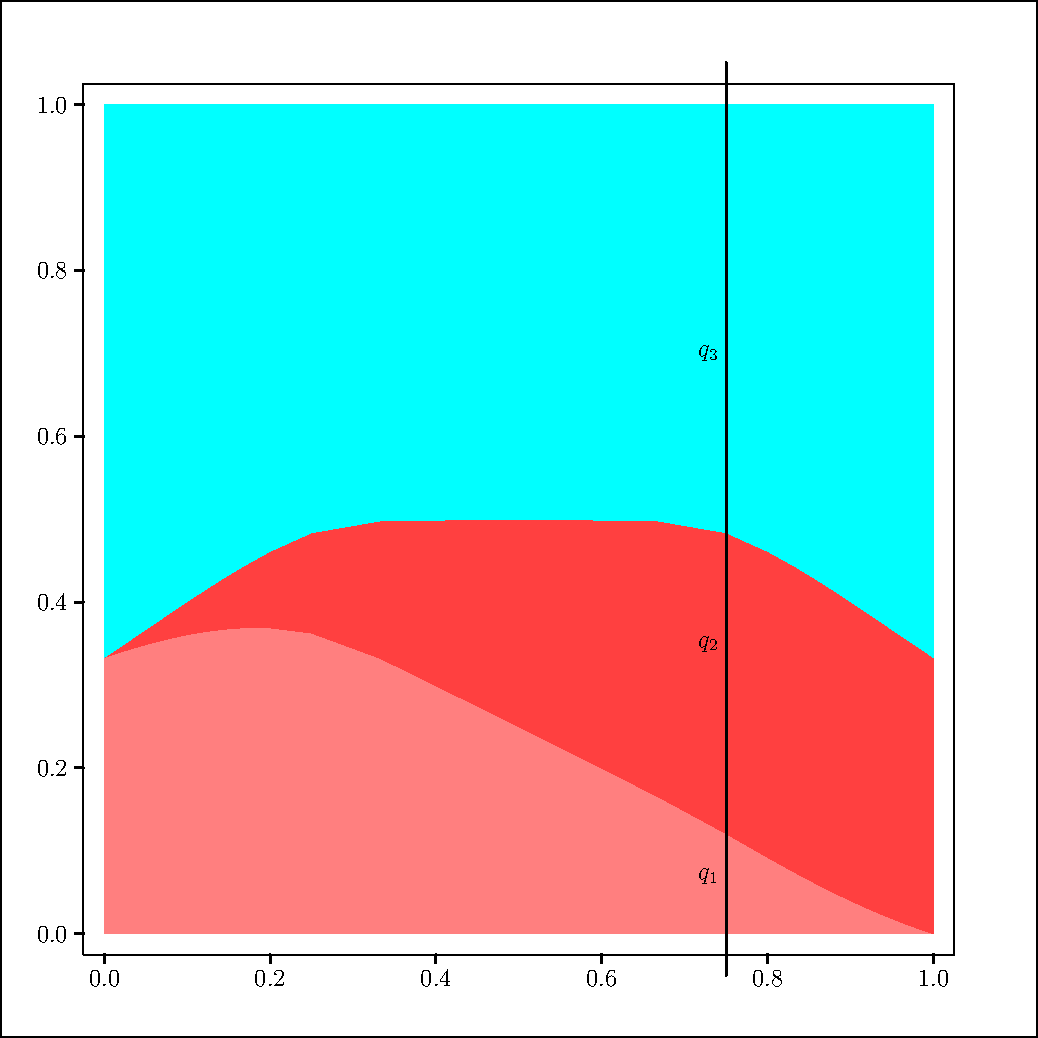
\includegraphics[scale=.4]{../diagrams/zeroone-pwst.pdf}
\end{figure}
\end{frame}

\begin{frame}
  \frametitle{Epistemic Entrenchment I}
  Sarah and Marian have arranged to go for sundowners at the
  Westcliff hotel tomorrow. Sarah feels there is some chance that
  it will rain, but thinks they can always enjoy the view from
  inside. To make sure, Marian consults the staff at the Westcliff
  hotel and finds out that in the event of rain, the inside area
  will be occupied by a wedding party. So she tells Sarah: ``If it
  rains tomorrow, we cannot have sundowners at the Westcliff.''
  Upon learning this conditional, Sarah sets her probability for
  sundowners and rain to zero, but she does not adapt her
  probability for rain.
\end{frame}

\begin{frame}
  \frametitle{Epistemic Entrenchment II}
  A jeweller has been shot in his store and robbed of a golden
  watch. However, it is not clear at this point what the relation
  between these two events is; perhaps someone shot the jeweller
  and then someone else saw an opportunity to steal the watch.
  Kate thinks there is some chance that Henry is the robber. On
  the other hand, she strongly doubts that he is capable of
  shooting someone, and thus, that he is the shooter. Now the
  inspector, after hearing the testimonies of several witnesses,
  tells Kate: ``If Henry robbed the jeweller, then he also shot
  him.'' As a result, Kate becomes more confident that Henry is
  not the robber, while her probability for Henry having shot the
  jeweller does not change.
\end{frame}

\begin{frame}
  \frametitle{Epistemic Entrenchment III}
  \begin{block}{Leaving the Antecedent Alone}
    ``In most cases the learning of a conditional is or would be
    irrelevant to one's degree of belief for the conditional's
    antecedent {\ldots} the learning of the relevant conditional
    should intuitively leave the probability of the antecedent
    unaltered.'' \linebreak (Douven and Romeijn)
  \end{block}
\end{frame}

\begin{frame}
  \frametitle{Coarsening at Random I}
  The CAR (Coarsening at Random) condition specifies when conditioning
  in a naive space works. A well-known example for conditioning in a
  naive space is the Monty Hall puzzle. We will consider Martin
  Gardner's Three Prisoners Puzzle, which is very similar.
  \begin{block}{The Three Prisoners Puzzle}
    Three men (A, B, and C) are under sentence of death when the
    governor decides to pardon one of them. The warden of the prison
    knows which of the three men is pardoned, but none of the men do.
    In a private conversation, A says to the warden, Tell me the name
    of one of the others who will be executed---it will not give
    anything away whether I will be executed or not. The warden agrees
    and tells A that B will be executed.
  \end{block}
\end{frame}

\renewcommand{\arraystretch}{2.1}
\begin{frame}
  \frametitle{Coarsening at Random II}
  \begin{table}
    \centering
    \begin{tabular}{|l|l|l|} \hline
      \rowcolor{myblue}\emph{observation} & \emph{update rule} & \emph{coincidence} \\ \hline
      \parbox{3cm}{\raggedright event and pairwise disjoint} & conditioning & always \\ \hline
      \parbox{3cm}{\raggedright event and arbitrary set} & conditioning & iff CAR holds \\ \hline
      \parbox{3cm}{\raggedright vector and partition} & Jeffrey conditioning & \parbox{3cm}{\raggedright iff generalization of CAR holds} \\ \hline
      \parbox{3cm}{\raggedright vector and no full \linebreak partition} & principle of \textsc{maxent} & \parbox{3cm}{\raggedright only in degenerate case} \\ \hline
    \end{tabular}
    \caption{Coincidence of naive and sophisticated conditioning}
  \end{table}
\end{frame}

\begin{frame}
  \frametitle{Coarsening at Random III}
  \begin{block}{CAR does not hold for Judy Benjamin}
    The set of observations for which [PME] conditioning
    corresponds to conditioning in the sophisticated space is a
    (Lebesgue) measure 0 set in the space of possible observations
    {\ldots} Seidenfeld shows that, under very weak conditions,
    [PME] updating cannot coincide with sophisticated conditioning
    if the observations have the form ``the conditional
    probability of $U$ given $V$ is $\alpha$ (as is the case in
    the Judy Benjamin problem). (Gr{\"u}nwald and Halpern)
  \end{block}
\end{frame}

\begin{frame}
  \frametitle{Coarsening at Random IV}
  \begin{figure}[h]
    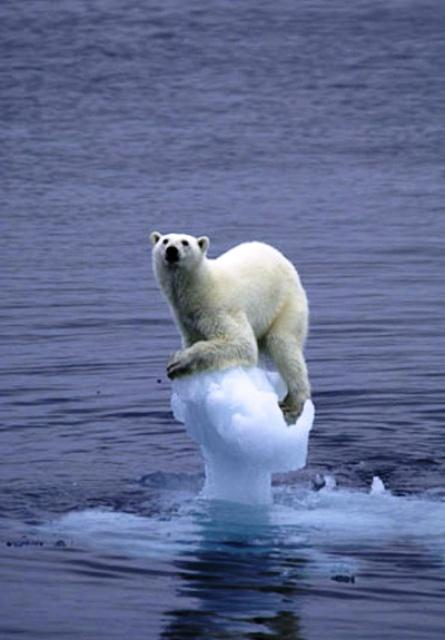
\includegraphics[scale=.25]{../diagrams/oh-no-global-warming.jpg}
  \end{figure}
\begin{center}
  This puts us in an awkward position.
\end{center}
\end{frame}

\begin{frame}
  \frametitle{Coarsening at Random V}
\begin{displaymath}
  P(\mbox{`A is pardoned'}|\mbox{`B will be
    executed'})=
\end{displaymath}
\begin{displaymath}
  \frac{P(\mbox{`A is pardoned'})}{P(\mbox{`A is
      pardoned'})+P(\mbox{`C is pardoned'})}=\frac{1}{2}\mbox{ (incorrect)}
\end{displaymath}
\end{frame}

\begin{frame}
  \frametitle{Coarsening at Random VI}
\begin{displaymath}
  P(\mbox{`A is pardoned'}|\mbox{`warden says B will be
    executed'})=
\end{displaymath}
\begin{displaymath}
  \frac{P(\mbox{`A is pardoned' and `warden says B will
      be executed'})}{P(\mbox{`warden says B will be
      executed'})}=
\end{displaymath}
\begin{displaymath}
  \frac{1/6}{1/2}=\frac{1}{3}\mbox{ (correct)}
\end{displaymath}
\end{frame}

\renewcommand{\arraystretch}{4}
\begin{frame}
  \frametitle{Coarsening at Random VII}
  \begin{table}
    \centering
    \begin{tabular}{|l|l|}\hline
    \rowcolor{myblue} \emph{Three Prisoners Puzzle} & \emph{Judy Benjamin Problem} \\ \hline
\parbox{3.5cm}{\raggedright naive space (informationally incorrect)} & \parbox{3.5cm}{\raggedright naive space} \\ \hline
\parbox{3.5cm}{\raggedright sophisticated space (informationally correct)} & \parbox{3.5cm}{\raggedright no sophisticated space without retrospective conditioning} \\ \hline
  \end{tabular}
    \caption{The disanalogy between the Three Prisoners and Judy Benjamin}
  \end{table}
\end{frame}

% \setbeamercolor{background canvas}{bg=black}
\begin{frame}
  \frametitle{End of Presentation}
% \begin{figure}[h]
%     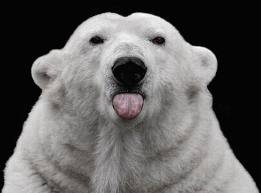
\includegraphics[scale=.4]{../diagrams/images.jpg}
%   \end{figure}
\end{frame}

\end{document}